\documentclass{article}

% Packages
\usepackage[utf8]{inputenc}
\usepackage[T1]{fontenc}
\usepackage{amsmath}
\usepackage{amssymb}
\usepackage{graphicx}
\usepackage{hyperref}
\usepackage{float}  
% Set smaller document margins
\usepackage[a4paper, margin=1in]{geometry}
\usepackage{hyperref}

% Customize nested itemize environments
\usepackage{enumitem}
% First set the global settings
\setlist[itemize]{leftmargin=*}
% Then set the level-specific settings
\setlist[itemize,1]{label=$\bullet$}
\setlist[itemize,2]{label=$\circ$, leftmargin=2em}
\setlist[itemize,3]{label=$\diamond$, leftmargin=3em}
% Bibliography management
\usepackage[numbers, super]{natbib}  % Better citation management with numbered references
\bibliographystyle{plainnat}  % Choose bibliography style
\usepackage{subcaption}  % Add this line to the preamble

% Document information
\title{Counterfactuals From the Penultimate Layer - Results Report}
\author{Conor Finlay}
\date{\today}

\begin{document}

\maketitle

\section{Introduction}

This document contains the results for some experiments which evaluate the use of Bayesian last-layer models for counterfactual explanations, generated from the penultimate layer representations of the model.

The model architecture remained the same for all experiments, only the Bayesian/non-Bayesian nature of the last-layer model was varied, as well as the training objective of the model. Details of the architecture can be found in Appendix \ref{appendix:model_architecture}.

\section{Uncertainty-reducing counterfactuals}
In this section, we evaluate the performance of each type of model on the task of generating uncertainty-reducing counterfactuals. There are 6 models in total, which are:

\begin{itemize}
    \item \textbf{Bayesian models}
    \begin{itemize}
        \item \textbf{Bayesian-C}: The Bayesian last-layer model trained with a classification-dominated objective.
        \item \textbf{Bayesian-A}: The Bayesian last-layer model trained with an autoencoder-dominated objective.
        \item \textbf{Bayesian-J}: The Bayesian last-layer model trained with a joint-objective.
    \end{itemize}
    \item \textbf{Non-Bayesian models}  
    \begin{itemize}
        \item \textbf{Deterministic-C}: The deterministic model trained with a classification-dominated objective.
        \item \textbf{Deterministic-A}: The deterministic model trained with an autoencoder-dominated objective.
        \item \textbf{Deterministic-J}: The deterministic model trained with a joint-objective.
    \end{itemize}
\end{itemize}


We identify fifty images from the MNIST test set which are classified with high entropy by the Bayesian-J model. A previous experiment involved using the fifty images each model was most uncertain about, but we found it more useful to compare a consistent set of images across all models.

On these fifty images, the models seek to generate counterfactuals which reduce the uncertainty of the model's prediction. This involves an optimisation within the penultimate layer space, inspired by CLUE\citep{clue}, which seeks to minimise both the entropy of the model's prediction and the distance between the original and counterfactual penultimate layer representations. This is expressed as:

\begin{equation}
    \min_{x'} \left( H(y|x') + \lambda \cdot \left\| x - x' \right\|_2 \right)
\end{equation}

where $x$ is the original image, $x'$ is the counterfactual, $y$ is the model's prediction, $H(y|x')$ is the entropy of the model's prediction, and $\lambda$ is a hyperparameter which balances the two terms.

In all of our experiments, we set $\lambda = 0.001$. 

\subsection{Qualitative Analysis}

\subsection{Entropy Reduction}

\begin{figure}[H]
    \centering
    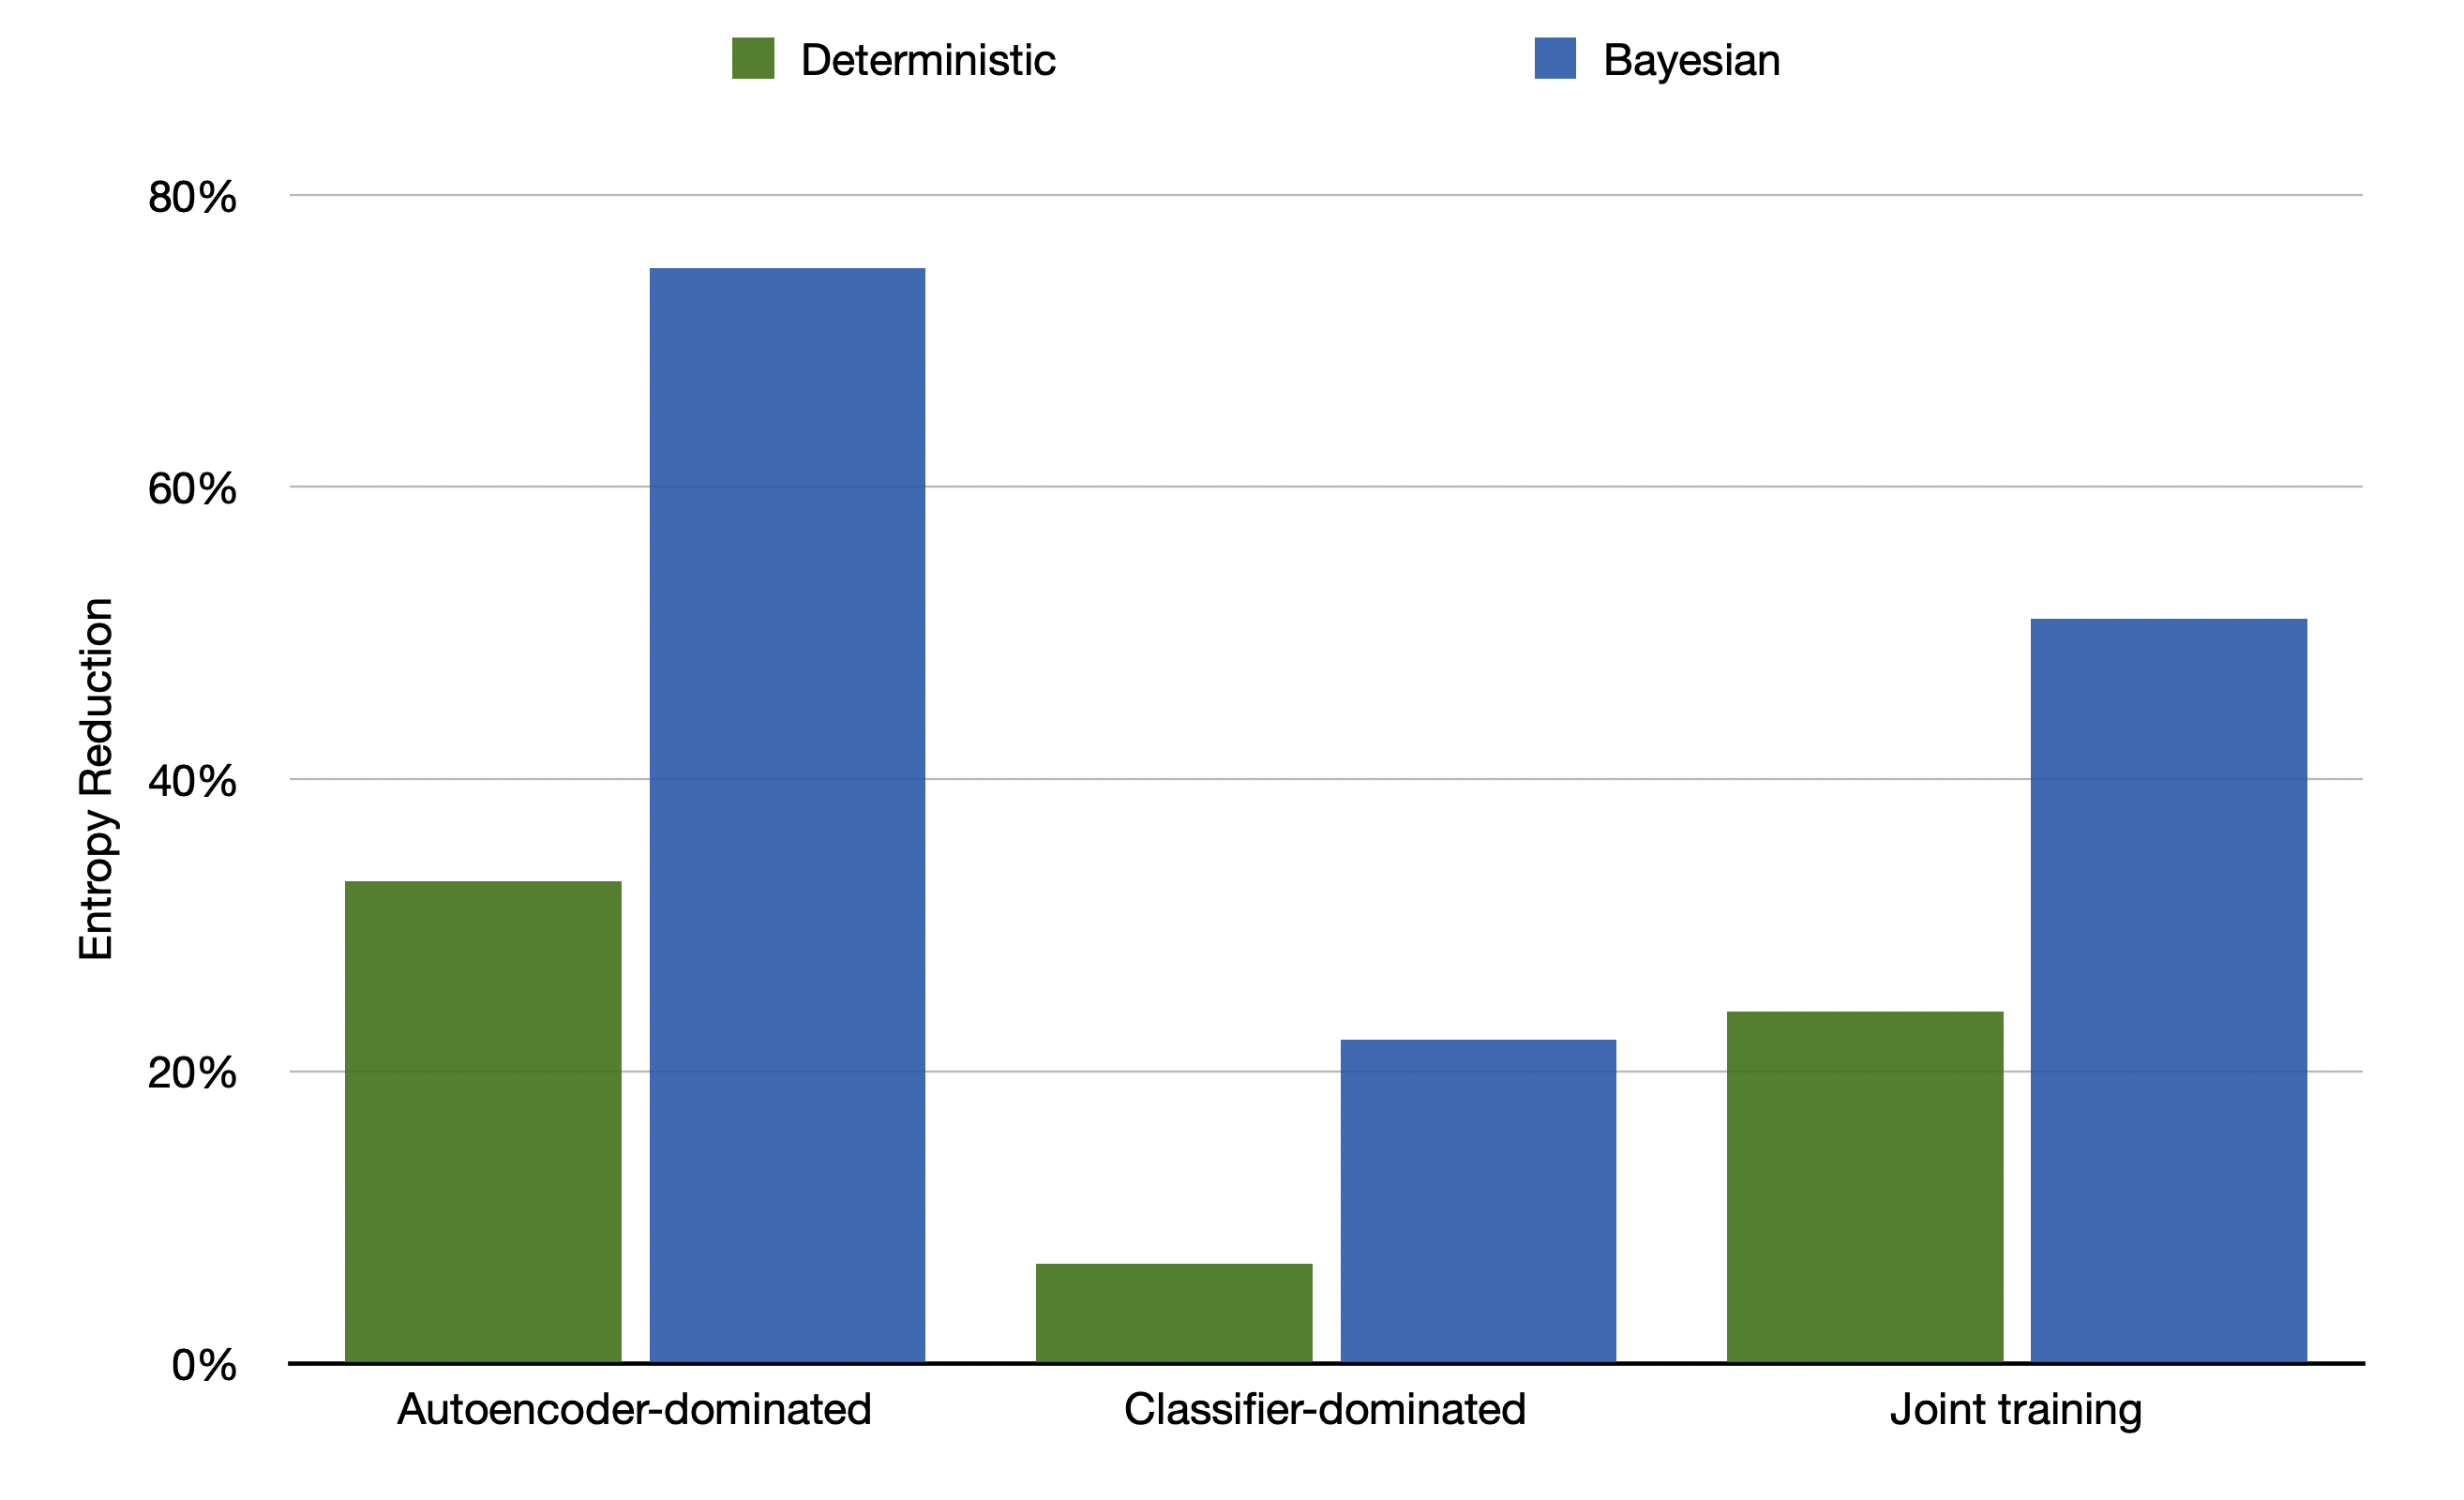
\includegraphics[width=0.6\textwidth]{figures/CLUE/EntropyReduction_Comparison.png}
    \caption{Comparison of the percentage entropy reduction of the models.}
    \label{fig:entropy_reduction}
\end{figure}


\subsection{Counterfactual Realism/Latent Space Distance}
\begin{figure}[H]
    \centering
    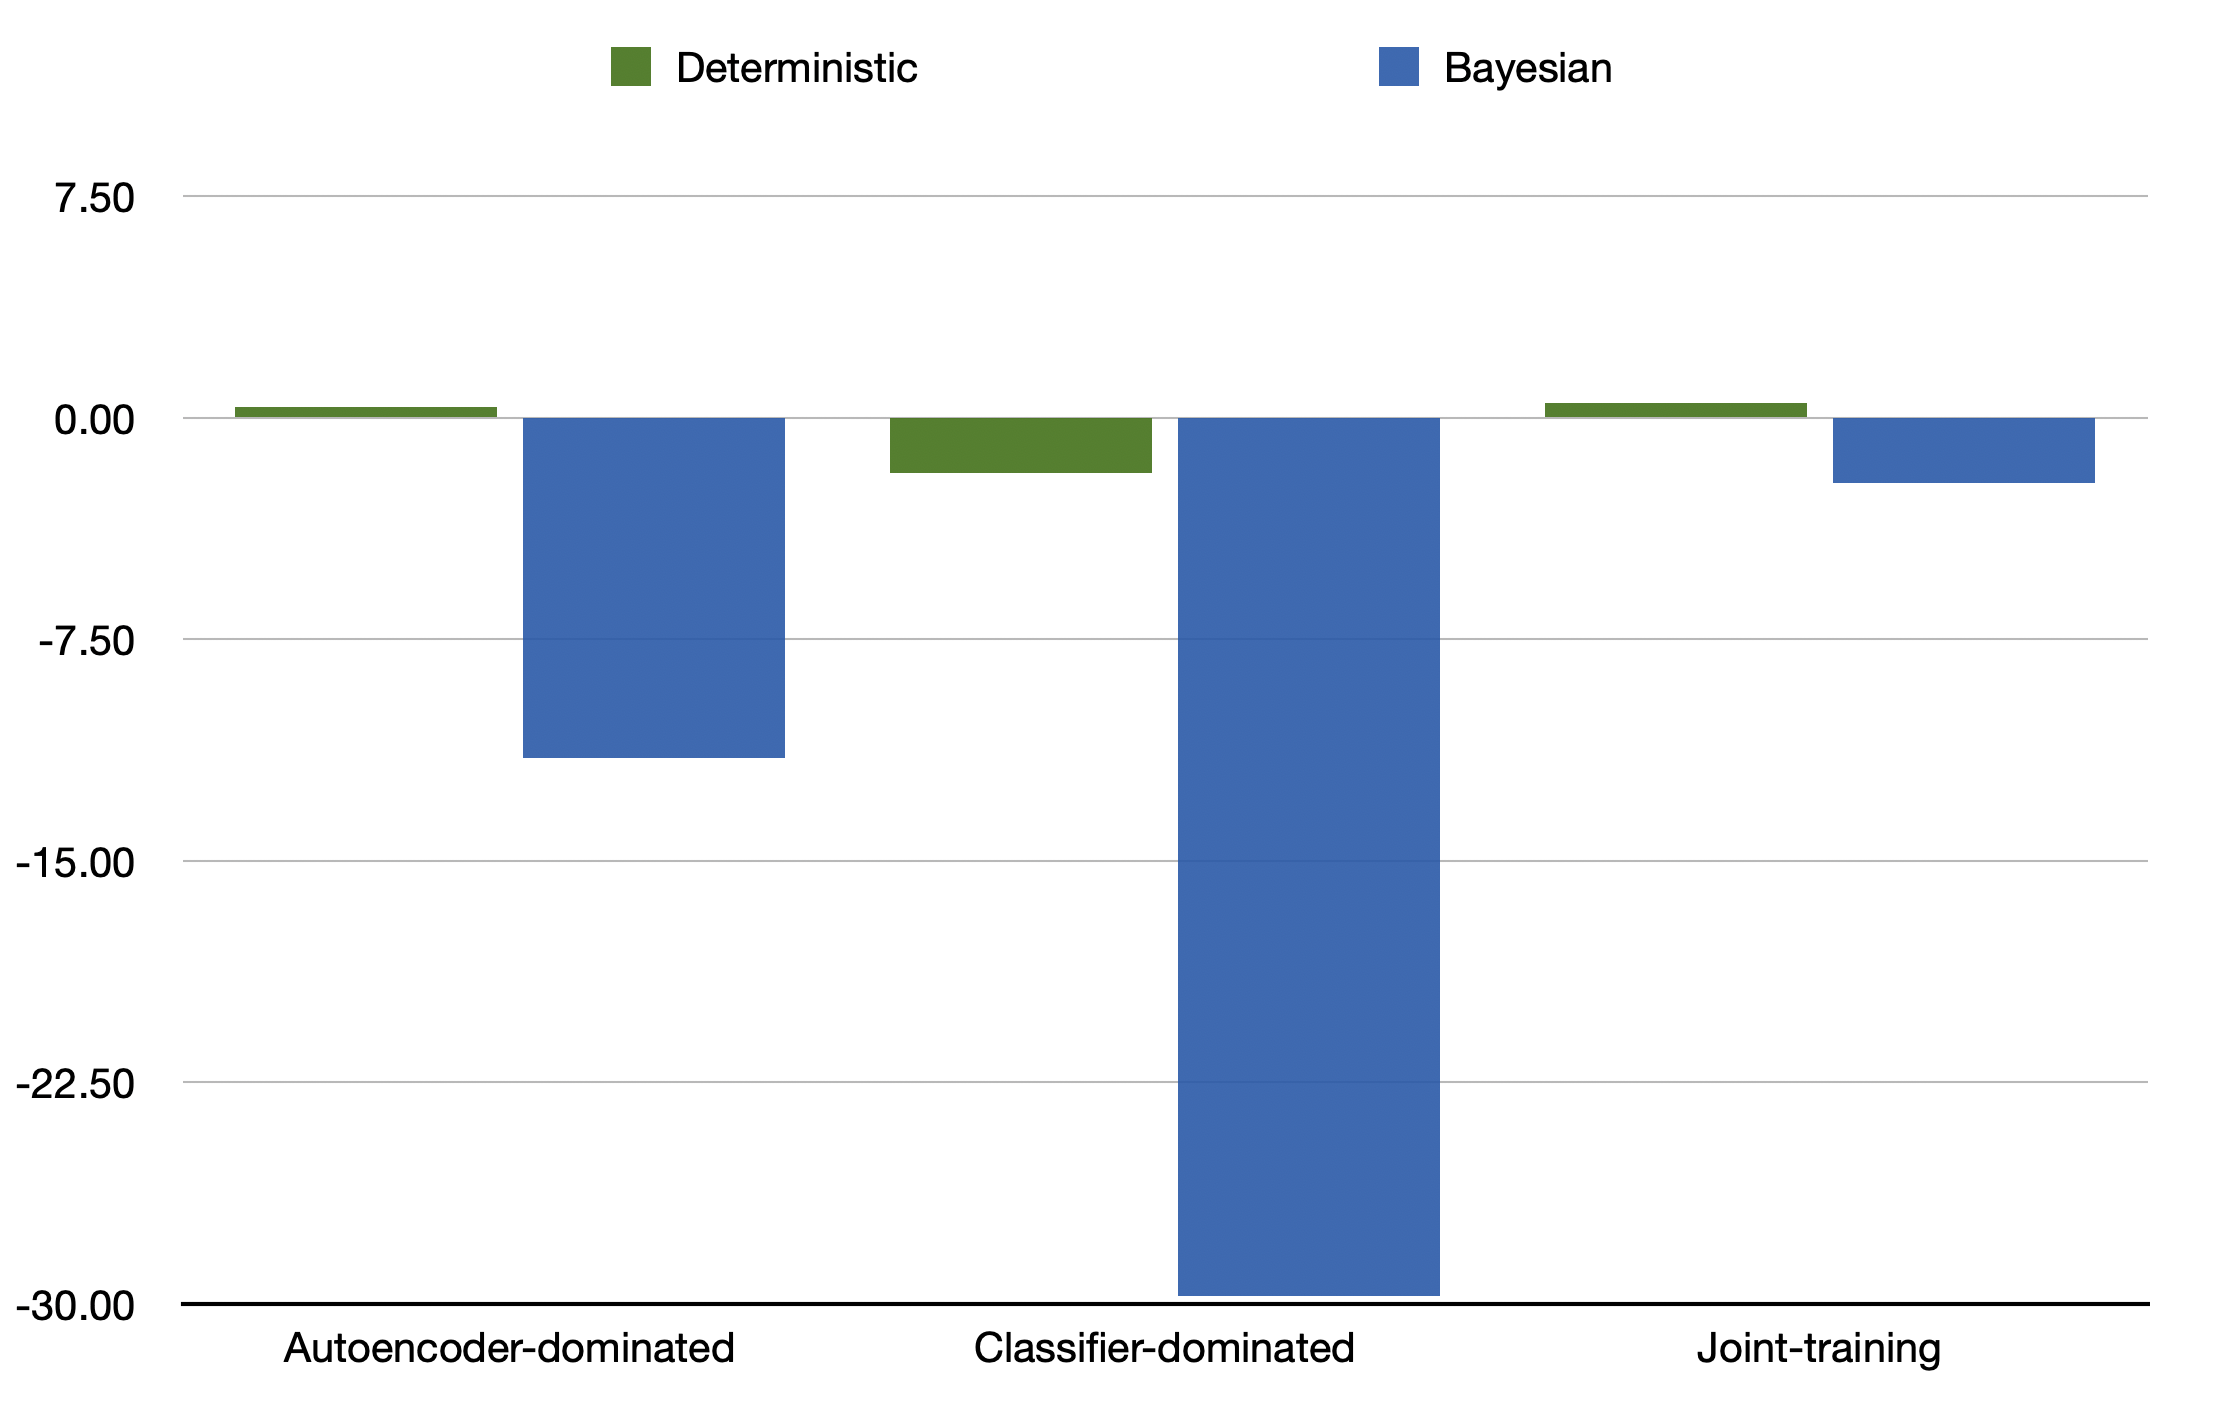
\includegraphics[width=0.6\textwidth]{figures/CLUE/CLUERealism.png}
    \caption{Comparison of the difference in realism between the original and counterfactual images.}
    \label{fig:counterfactual_realism}
\end{figure}

\begin{figure}[H]
    \centering
    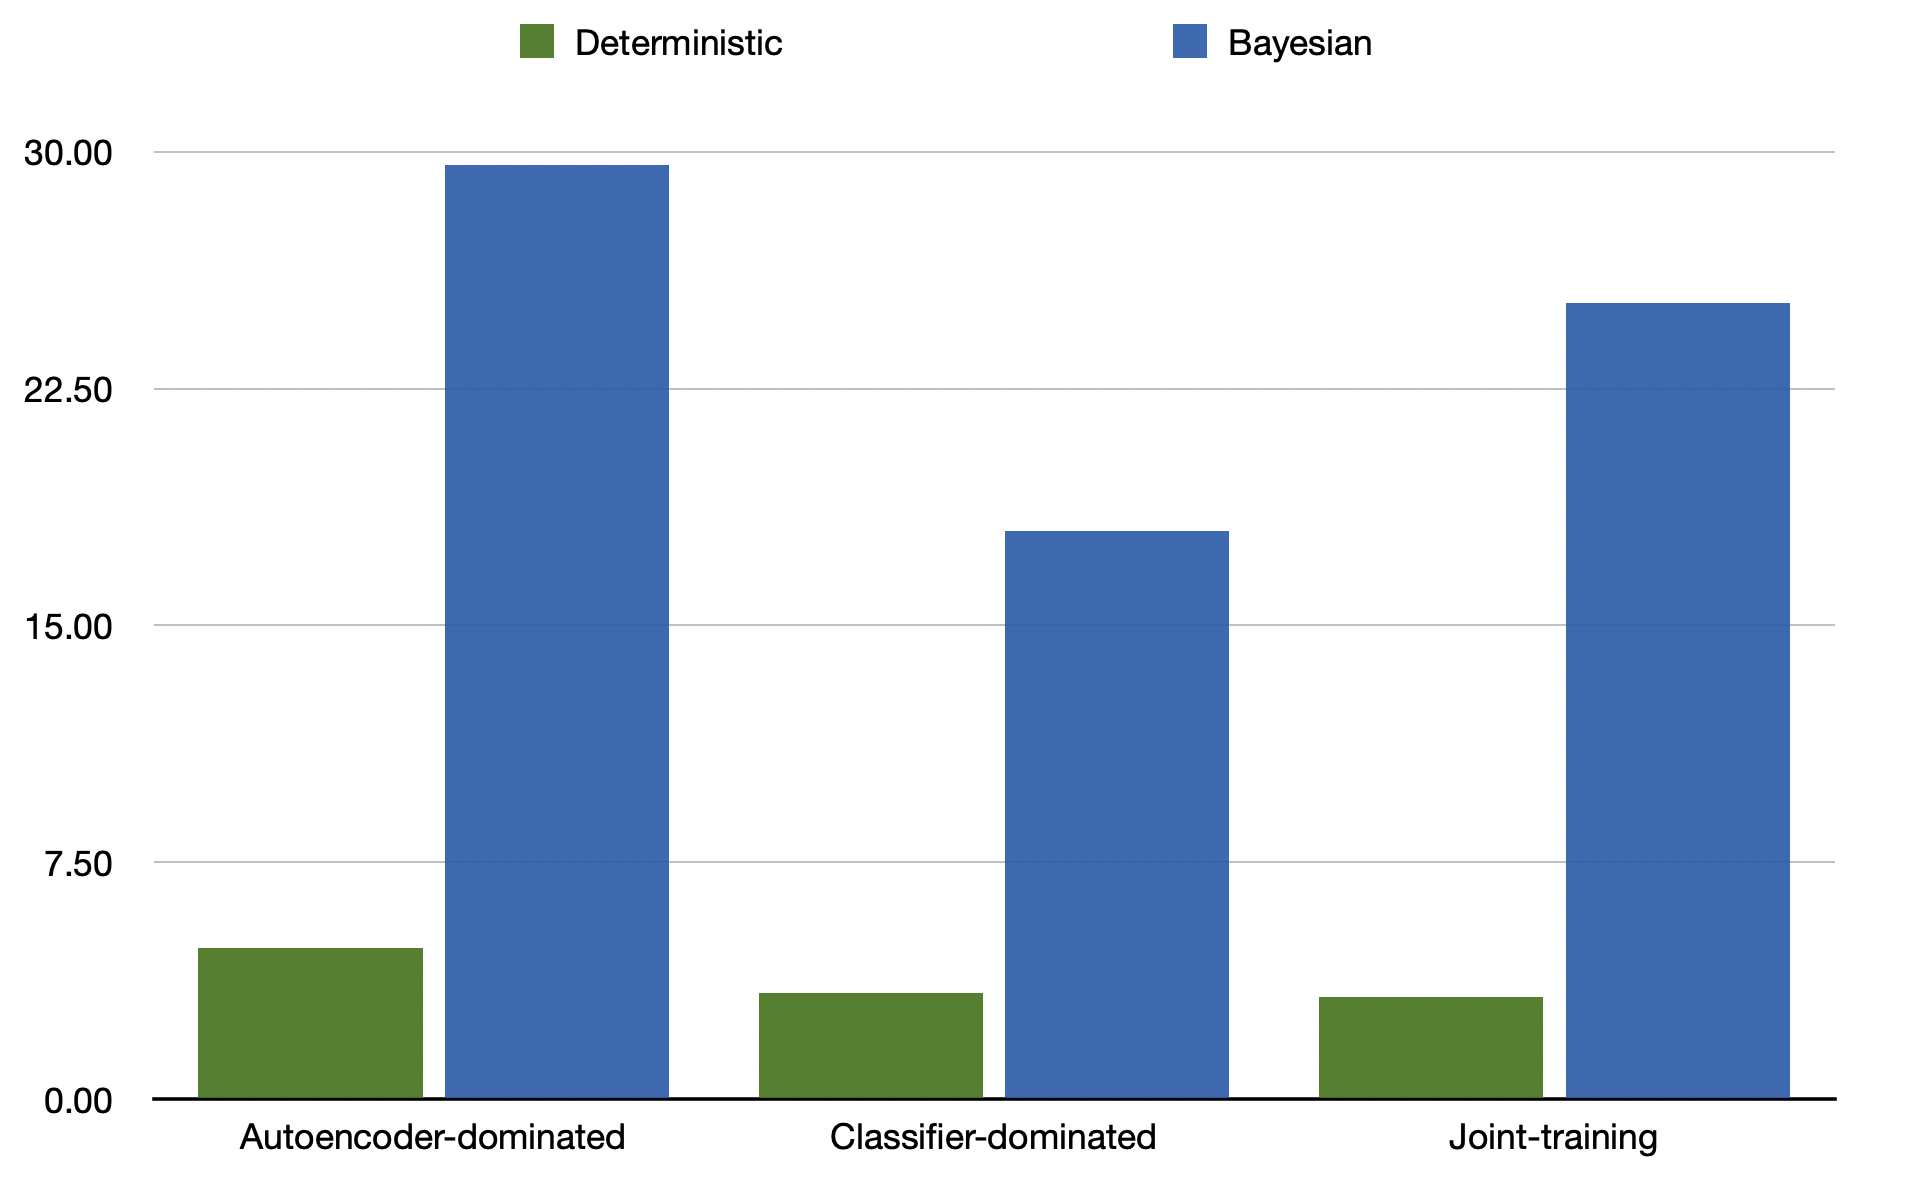
\includegraphics[width=0.6\textwidth]{figures/CLUE/CLUELatentDistance.png}
    \caption{Comparison of the latent space distance between the original and counterfactual images.}
    \label{fig:counterfactual_latent_distance}
\end{figure}


\subsection{Class Consistency}

\begin{figure}[H]
    \centering
    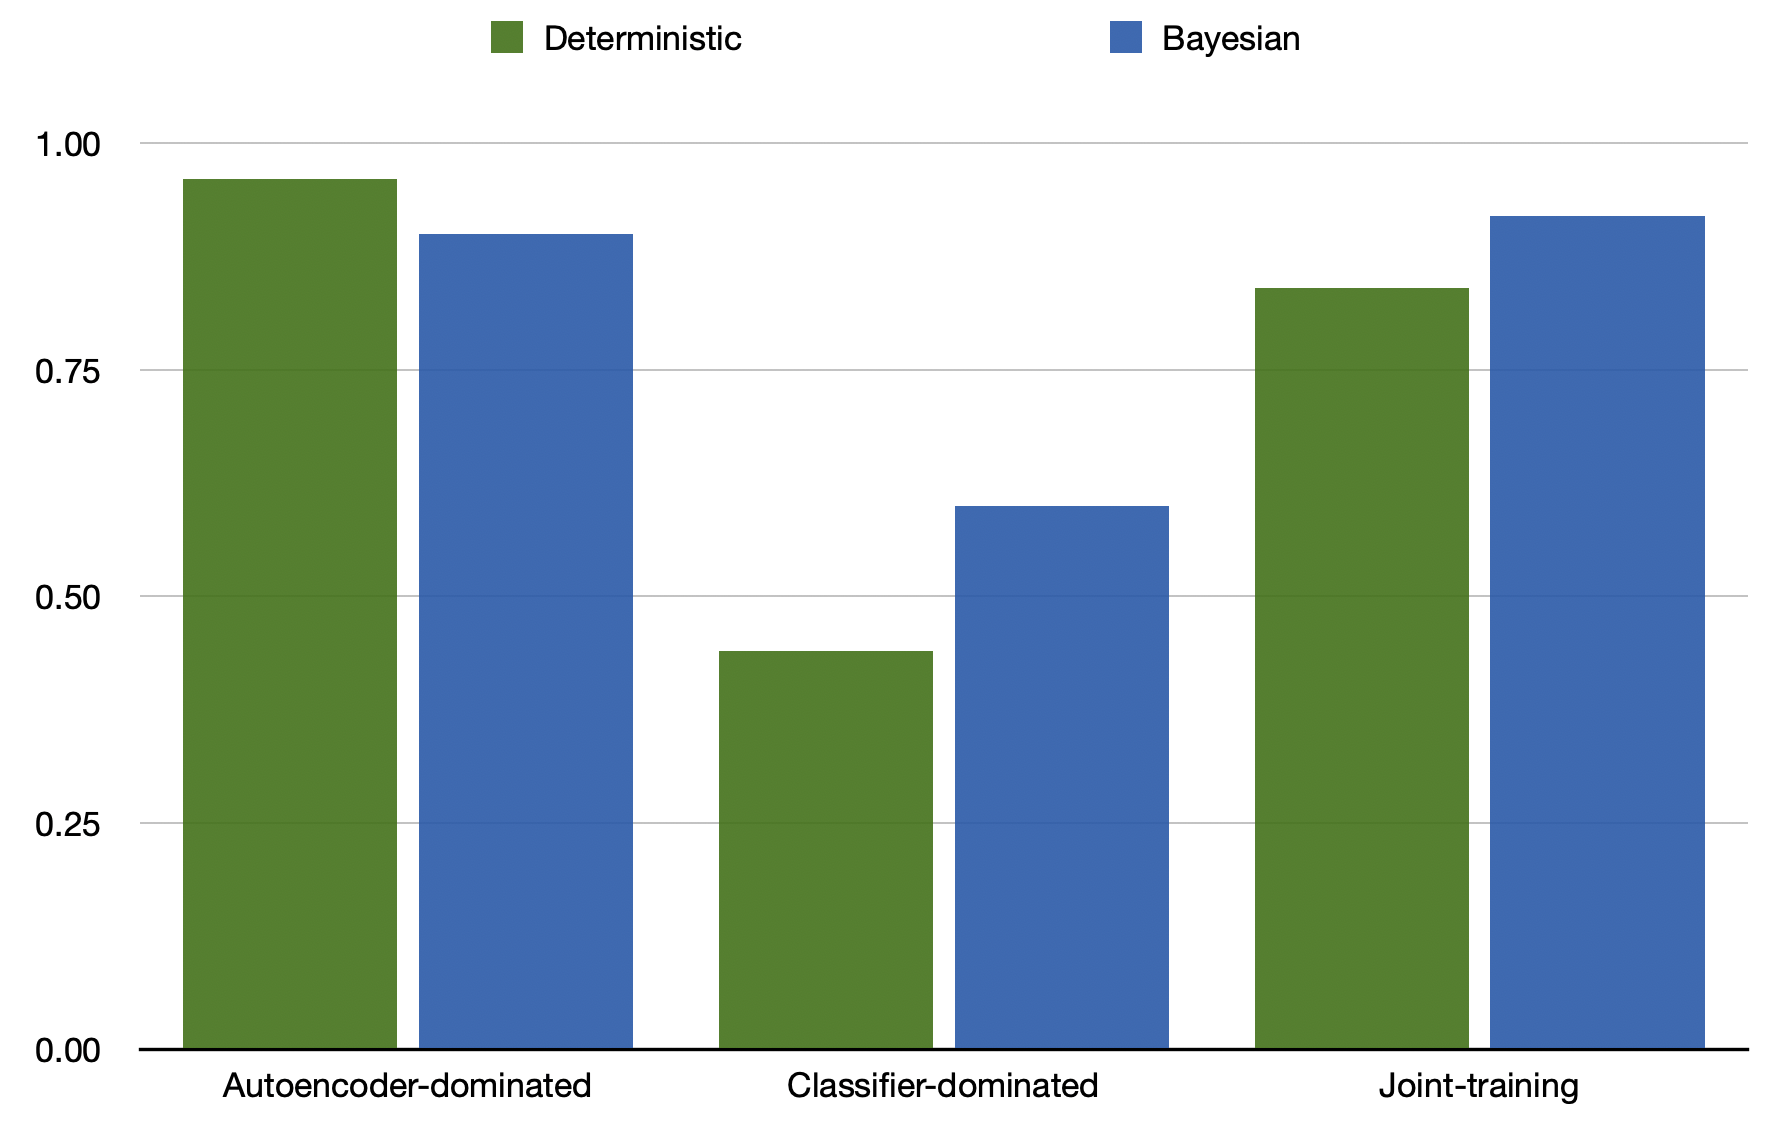
\includegraphics[width=0.6\textwidth]{figures/CLUE/ClassConsistency.png}
    \caption{Comparison of the class consistency.}
    \label{fig:class_consistency}
\end{figure}

\section{Class-changing counterfactuals}

In this section, we evaluate the performance of each type of model on the task of generating class-changing counterfactuals. That is, we specify a target class that differs from the original class of an image, and optimisation attempts to find a minimal change (in latent space) which changes the class prediction to the target class.

As a result, the new optimisation problem is:

\begin{equation}
    \max_{x'} \left( \hat{y}_{\text{target}}(x') - \lambda \cdot \left\| x - x' \right\|_2 \right)
\end{equation}

where $x$ is the original image, $x'$ is the counterfactual, $\hat{y}_{\text{target}}(x')$ is the softmax prediction confidence of the target class, and $\lambda$ is a hyperparameter which balances the two terms.


\subsection{Qualitative Analysis}
\subsubsection{Example 1: 9 \texorpdfstring{$\rightarrow$}{to} 8}

\begin{figure}[H]
    \centering
    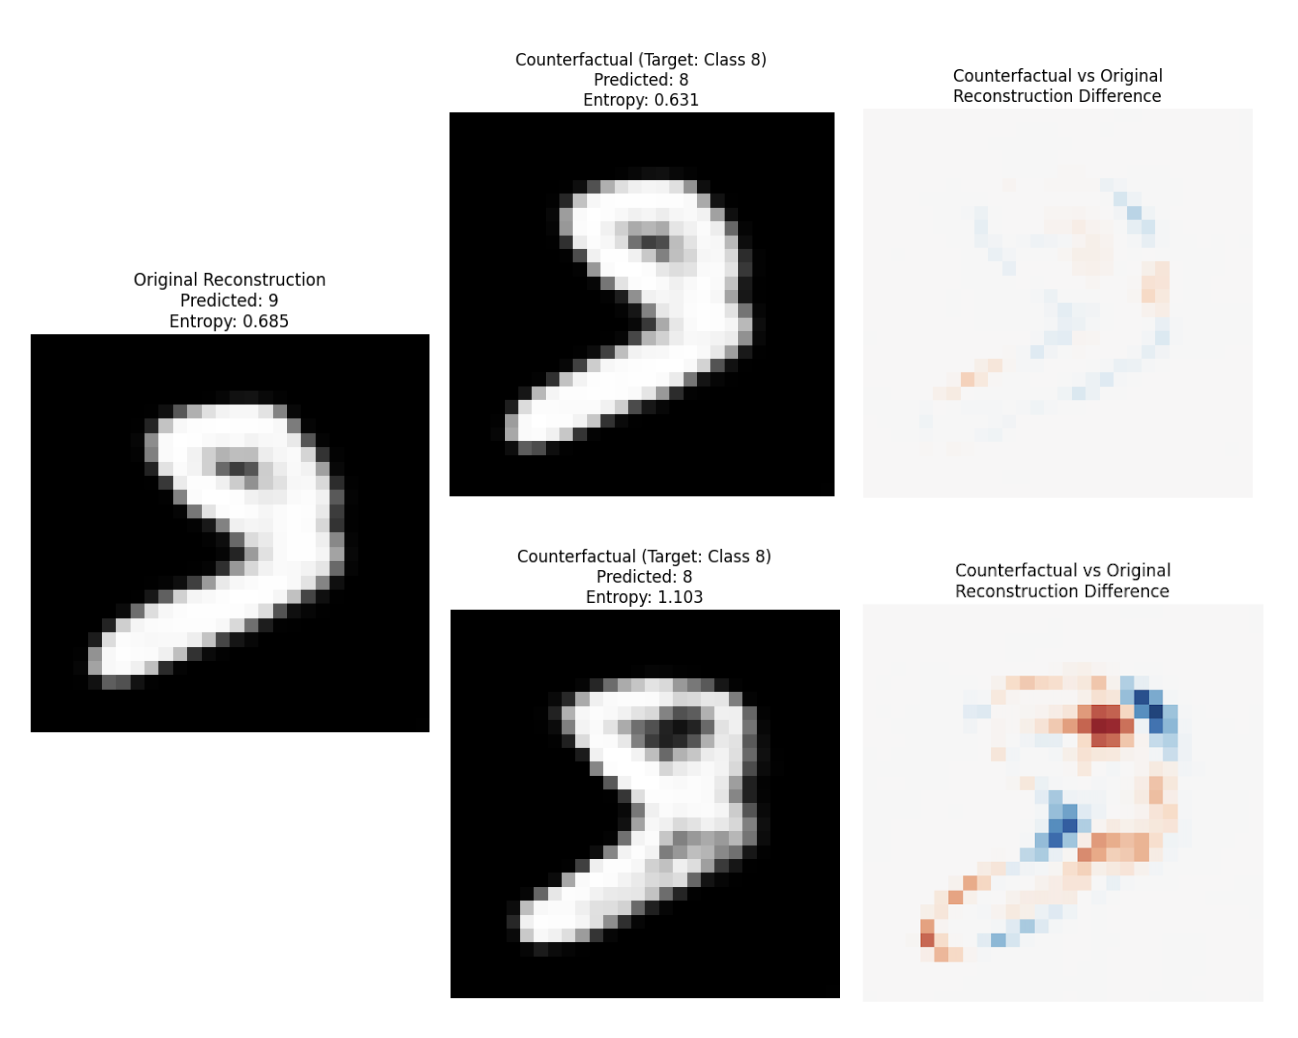
\includegraphics[width=0.6\textwidth]{figures/Class/9to8_comparison.png}
    \caption{Comparison of the class-changing counterfactuals from 9 to 8 (top: deterministic, bottom: Bayesian).}
    \label{fig:cc_qualitative_9to8}
\end{figure}



\begin{figure}[H]
    \centering
    \begin{subfigure}{0.48\textwidth}
        \centering
        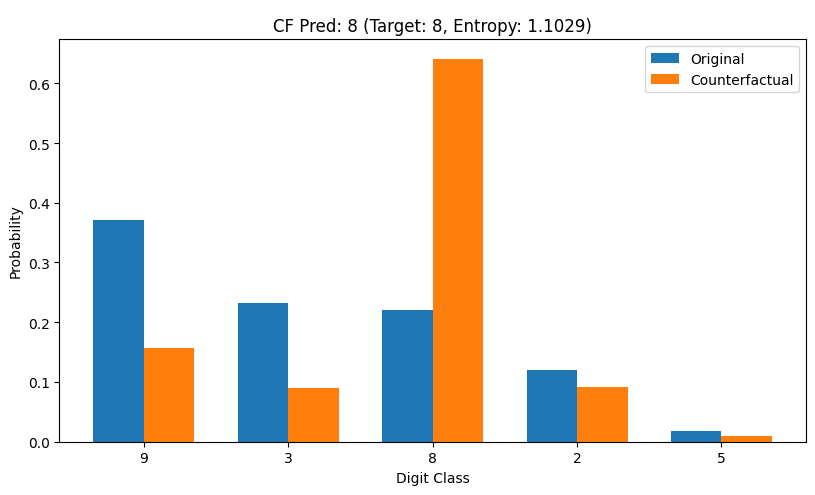
\includegraphics[width=\textwidth]{figures/Class/9to8_Bayes_distribution.png}
        \caption{Bayesian model.}
        \label{fig:cc_qualitative_bayesian_9to8}
    \end{subfigure}
    \hfill
    \begin{subfigure}{0.48\textwidth}
        \centering
        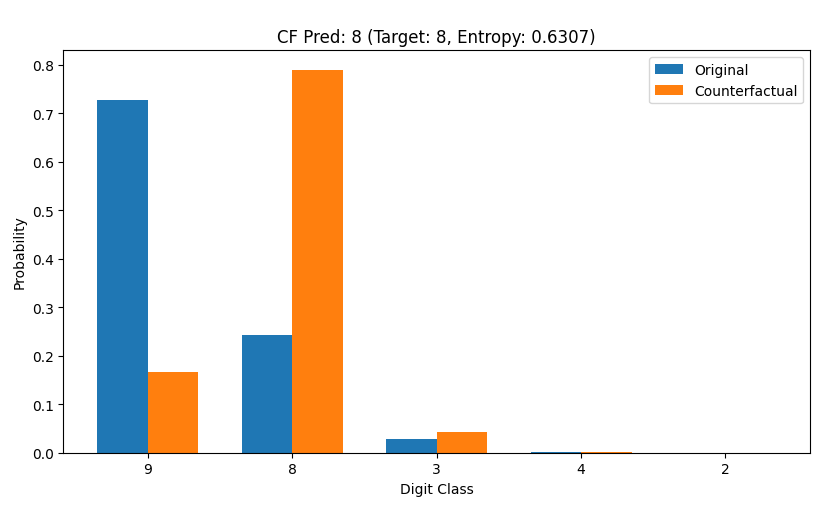
\includegraphics[width=\textwidth]{figures/Class/9to8_Det_distribution.png}
        \caption{Deterministic model.}
        \label{fig:cc_qualitative_det_9to8}
    \end{subfigure}
    \caption{Softmax outputs before and after counterfactual optimisation ($9 \rightarrow 8$).}
    \label{fig:cc_qualitative_distribution_9to8}
\end{figure}




\subsection{Target Class Confidence}

\begin{figure}[H]
    \centering
    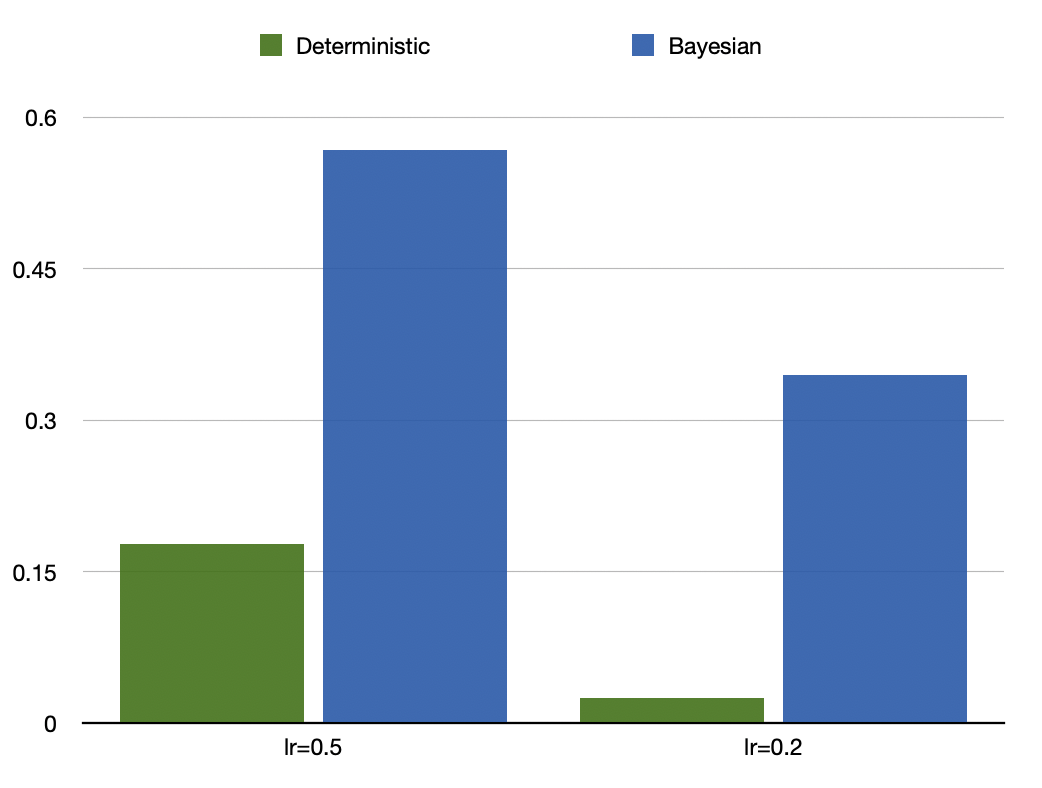
\includegraphics[width=0.6\textwidth]{figures/Class/ConfidenceIncrease.png}
    \caption{Target class confidence increase for class-changing counterfactuals (reconstructions).}
    \label{fig:cc_confidence_increase}
\end{figure}

\begin{table}[H]
    \centering
    \begin{tabular}{|c|c|c|c|}
        \hline
        & Learning rate & Distance weight & Steps \\
        \hline
        Params 1 (aggressive learning rate) & 0.5 & 0.001 & 200 \\
        \hline
        Params 2 (lower learning rate) & 0.2 & 0.001 & 200 \\
        \hline
    \end{tabular}
    \caption{Parameter settings with different learning rates.}
    \label{tab:parameter_settings}
\end{table}

\begin{table}[H]
    \centering
    \begin{tabular}{|c|c|c|}
        \hline
        & Deterministic & Bayesian \\
        \hline
        Params 2 & 0.580 & 0.974 \\
        \hline
    \end{tabular}
    \caption{Target class confidence increase in latent space (pre-reconstruction).}
    \label{tab:target_class_confidence_latent}
\end{table}

Looking at \autoref{tab:target_class_confidence_latent}, we see that the average target class confidence increase during optimisation (before reconstruction) is only 0.58 for deterministic model. In practice, this is not because in most instances the figure is around that value. Instead, in each instance, the optimisation either succeeds, in which case the target class confidence is 1.0, or it fails, in which case the target class confidence is 0.0. As such, the 0.58 figure indicates that the optimisation fairs 42\% of the time for a learning rate of 0.2. 

Although the learning rate has an effect on the Bayesian model's optimisation, it is more continuous and never results in failed optimisation. We explore this in the following section.



\subsection{Optimisation}

In \autoref{fig:optimisation}, we plot the target class confidence during optimisation for the deterministic and Bayesian models. This shows the stark contrast between the counterfactual optimisation between the two models. 

\begin{figure}[H]
    \centering
    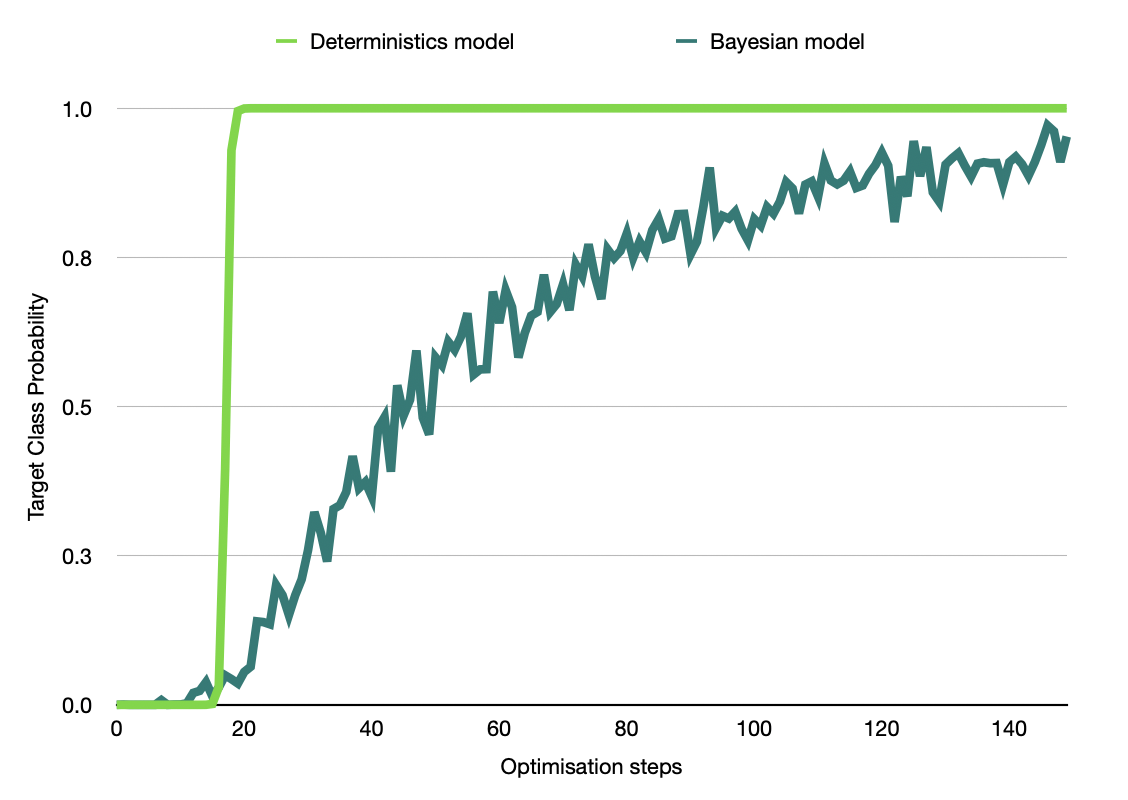
\includegraphics[width=0.6\textwidth]{figures/Class/Optimisation.png}
    \caption{Target class confidence during optimisation.}
    \label{fig:optimisation}
\end{figure}

The optimisation for the Bayesian model makes near instant progress, and proceeds gradually to maximise the target class confidence. On the other hand, the deterministic model's optimisation makes no progress for about 15 steps, before suddenly reaching full target class confidence. 

This sheds light on why the counterfactual optimisation for the deterministic model is so unstable. Loosely speaking, the optimisation stumbles around 'blindly' until it comes across a region in latent space for which the target class is predicted, and stays there for the rest of the optimisation. If it never comes across such a region, the optimisation fails. In particular, if there is any significant weight placed on the distance term in the objective function, the optimisation frequently fails as any exploration only serves to increase the value of the loss function. 



\label{appendix:model_architecture}

\subsection{Model Architecture}
The base architecture follows the ReGene approach ("Classify and Generate"), which consists of two main components:

\begin{itemize}
    \item \textbf{Classifier}: A convolutional neural network with the following structure:
    \begin{itemize}
        \item Three convolutional blocks, each containing:
        \begin{itemize}
            \item Convolutional layer
            \item Batch normalization
            \item ReLU activation
            \item Max pooling
        \end{itemize}
        \item Flattening layer
        \item Linear projection to latent space (dimension 128)
        \item Final classification layer
    \end{itemize}
    
    \item \textbf{Decoder}: A network that reconstructs images from the latent representations:
    \begin{itemize}
        \item Linear projection from latent space to match flattened dimensions
        \item Three transposed convolutional blocks for upsampling
        \item Final sigmoid activation for pixel values
    \end{itemize}
\end{itemize}

The architecture allows for different training objectives:
\begin{itemize}
    \item \textbf{Classification-dominated training}: The classifier portion of the model (and therefore the encoder) is trained to maximise classification accuracy only. The decoder is then trained to reconstruct the training image from the penultimate layer representations of the frozen classifier.
    \item \textbf{Autoencoder-dominated training}: The encoder (classification backbone) and decoder are trained jointly to minimise the reconstruction loss between the input and output images. A single classification head is then trained to maximise classification accuracy on the training set, while taking the embeddings from the frozen encoder.
    \item \textbf{Joint-objective training}: The encoder, decoder and classification head are trained jointly to minimise a loss function which balances the classification accuracy and the reconstruction loss. The encoder balances the classification and reconstruction loss by weighting the two loss terms, while the decoder naturally only minimises the reconstruction loss, and the classification head only the classification loss.
\end{itemize}

\subsection{Bayesian Last Layer (BLL-VI)}
For the Bayesian variant, we replace the final classification layer with a Bayesian linear layer:

\begin{itemize}
    \item \textbf{Backbone}: The pretrained convolutional network up to the penultimate layer
    \item \textbf{Bayesian Last Layer}: A variational inference-based Bayesian linear layer with:
    \begin{itemize}
        \item Gaussian prior on weights (configurable mean and standard deviation)
        \item Learnable posterior distributions for weights
        \item KL divergence regularization during training
    \end{itemize}
\end{itemize}

The BLL-VI model provides:
\begin{itemize}
    \item Uncertainty quantification through multiple forward passes (Monte Carlo sampling)
    \item Decomposition of uncertainty into aleatoric (data) and epistemic (model) components
    \item Ability to generate predictions directly from latent representations
\end{itemize}

During training, the backbone remains frozen while only the Bayesian last layer is optimized, using a loss function that combines cross-entropy and KL divergence terms.

\bibliography{references}

\end{document}
